\documentclass[a4paper]{article}

%% Language and font encodings
\usepackage[english]{babel}
\usepackage[utf8x]{inputenc}
\usepackage[T1]{fontenc}

%% Sets page size and margins
\usepackage[a4paper,top=3cm,bottom=2cm,left=3cm,right=3cm,marginparwidth=2cm]{geometry}

%% Useful packages
\usepackage{amsmath}
\usepackage{amsfonts}
\usepackage{bbm}
\usepackage{graphicx}
\usepackage[colorinlistoftodos]{todonotes}
\usepackage[colorlinks=true, allcolors=blue]{hyperref}
\usepackage{float}
\usepackage{enumerate}
\usepackage{mathrsfs}
\usepackage{subcaption}

\usepackage{tikz}
\tikzset{
    vertex/.style={circle,draw,minimum size=1.5em},
    edge/.style={->,> = latex'}
}

\title{Stochastic Processes}
\author{Kevin Chang}

\graphicspath{ {./images/} }

\begin{document}
\maketitle

\section{}
\begin{itemize}
\begin{figure} [H]
    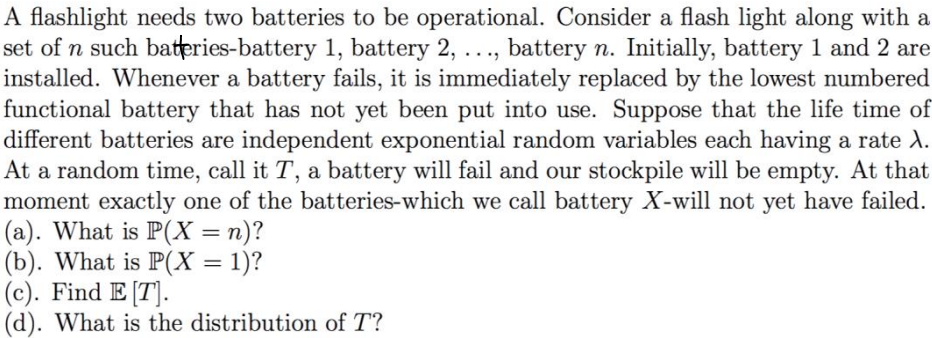
\includegraphics[width=1\linewidth]{question/1.png}
\end{figure}
    \item Consider the process as one Poisson process with $2 \lambda$ and split the process with $p = \frac{1}{2}$
    \item (a) $P[X=n]$
        \begin{itemize}
            \item as long as $n-1$-th fail and $n-2$-th fail are in different batteries holder $\rightarrow X = n$
            \item $P[X=n] = \frac{1}{2}$
        \end{itemize}
    \item (b)
        \begin{itemize}
            \item $P[X=1] = (\frac{1}{2})^{n-1}$
        \end{itemize}
    \item (c)
        \begin{itemize}
            \item $\mathbb{E}[T] = \frac{n-1}{\lambda}$
        \end{itemize}
    \item (d)
        \begin{itemize}
            \item a Poisson distribution
        \end{itemize}
\end{itemize}

\section{}
\begin{itemize}
\begin{figure} [H]
    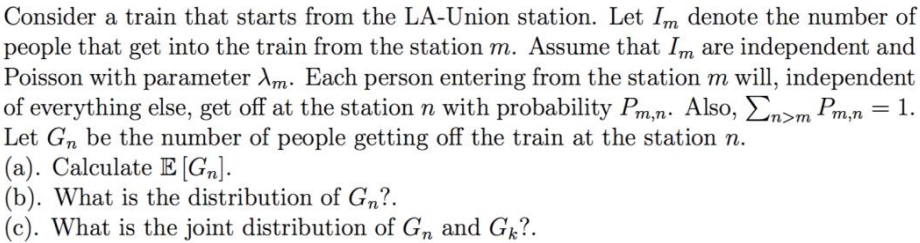
\includegraphics[width=1\linewidth]{question/2.png}
\end{figure}
    \item $G_n$ is a Poisson process with $\lambda = \sum_{i = 0}^{n-1} \lambda_m \times P_{m,i}$
    \item (a)
        \begin{itemize}
            \item $\mathbb{E}[G_n] = \sum_{i = 0}^{n-1} \lambda_m \times P_{m,i}$
        \end{itemize}
    \item (b)
        \begin{itemize}
            \item $G_n$ is a Poisson process with $\lambda = \sum_{i = 0}^{n-1} \lambda_m \times P_{m,i}$
        \end{itemize}
    \item (c)
        \begin{itemize}
            \item $G_n$ and $G_k$ is indepedent
            \item $G_n$ is a Poisson process with $\lambda_n = \sum_{i = 0}^{n-1} \lambda_m \times P_{m,i}$
            \item $G_k$ is a Poisson process with $\lambda_k = \sum_{i = 0}^{k-1} \lambda_m \times P_{m,i}$
            \item $F_{G_n, G_k}(i, j) = \frac{\lambda_n^i}{i!}\exp(-\lambda_n) \times \frac{\lambda_k^j}{j!}\exp(-\lambda_k)$
        \end{itemize}
\end{itemize}

\section{}
\begin{itemize}
\begin{figure} [H]
    
\includegraphics[width=1\linewidth]{question/3.png}
\end{figure}
    \item Suppose $B$ is the time the bus arrived at the stop
    \item Suppose $T$ is the time to reach home
    \item (a)
        \begin{itemize}
            \item $\mathbb{E}[T] = (W + s)\times P[B > s] + \int_0^s (R+t) \lambda e^{-\lambda t} dt$

                $= (W + s)e^{-\lambda s} + R (1 - e^{-\lambda s}) + \frac{1}{\lambda} + e^{-\lambda s} (-s + \frac{-1}{\lambda})$

                $= (W - R - \frac{1}{\lambda}) e^{-\lambda s} + R + \frac{1}{\lambda}$
        \end{itemize}
    \item (b)
        \begin{itemize}
            \item $\frac{d \mathbb{E}[T]}{ds} = (W - R - \frac{1}{\lambda}) \times (-\lambda)e^{-\lambda s}$
            \item if $(W - R - \frac{1}{\lambda}) < 0$, $\mathbb{E}[T]$ increases when $s$ increases $\rightarrow$ minimum happens when $s=0$
            \item if $(W - R - \frac{1}{\lambda}) > 0$, $\mathbb{E}[T]$ decreases when $s$ increases $\rightarrow$ minimum happens when $s=\infty$
            \item if $(W - R - \frac{1}{\lambda}) = 0$, the derivative of $\mathbb{E}[T]$ is constant $\rightarrow$ minimum happens for any $s$
        \end{itemize}
    \item (c)
        \begin{itemize}
            \item since the exponential distribution is memoryless, if $\mathbb{E}[T]$ is minimized when $s = t$, then, at $s=t$, $\mathbb{E}[T]$ is minimized when $s = t + t = 2t$. Therefore, $t = \infty$
        \end{itemize}
\end{itemize}

\section{}
\begin{itemize}
\begin{figure} [H]
    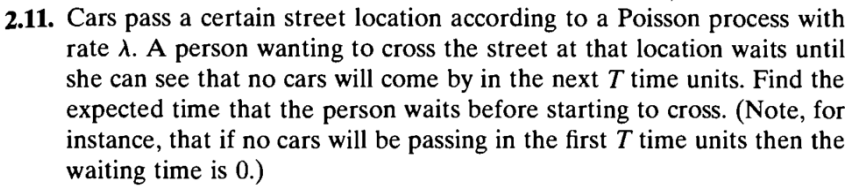
\includegraphics[width=1\linewidth]{question/4.png}
\end{figure}
    \item $X_i$: waiting time for $i$-th bus
    \item $N$: number of cars the person has to wait
    \item $P$: the time that the person has to wait
    \item $P[N=n] = (e^{-\lambda T})(1-e^{-\lambda T})^n$
    \item $\mathbb{E}[P|N=n] = n \times \mathbb{E}[X_i|X_i < T] + \mathbb{E}[X_i|X_i>T]$

        $= n(-Te^{-\lambda T} + \frac{1-e^{-\lambda T}}{\lambda}) + Te^{-\lambda T} + \frac{e^{-\lambda T}}{\lambda}$
        $= (1-n)(Te^{-\lambda T} + \frac{e^{-\lambda T}}{\lambda}) + \frac{n+1}{\lambda}$
    \item $\mathbb{E}[P] = \sum_{n = 0}^\infty \mathbb{E}[P|N=n] P[N=n]$

        $= \sum_{n = 0}^\infty \mathbb{E}[P|N=n] P[N=n]$

        $= (1-\frac{1-e^{-\lambda T}}{e^{-\lambda T}})(Te^{-\lambda T} + \frac{e^{-\lambda T}}{\lambda}) + \frac{1}{\lambda e^{-\lambda T}}$

        $= (\frac{2e^{-\lambda T} - 1}{e^{-\lambda T}})(Te^{-\lambda T} + \frac{e^{-\lambda T}}{\lambda}) + \frac{1}{\lambda e^{-\lambda T}}$
\end{itemize}

\section{}
\begin{itemize}
\begin{figure} [H]
    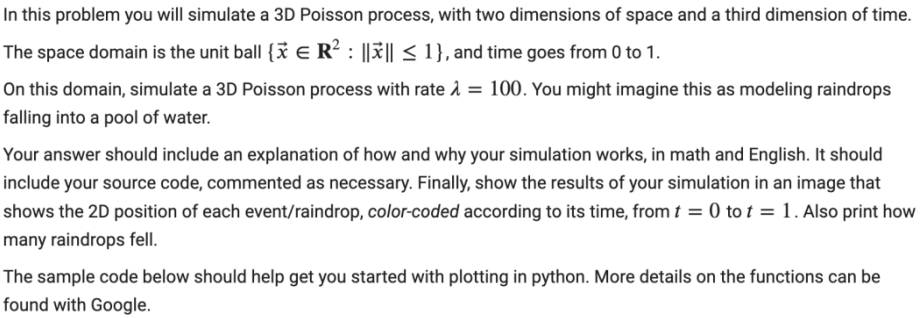
\includegraphics[width=1\linewidth]{question/5.png}
\end{figure}
    \item Code
\begin{figure} [H]
    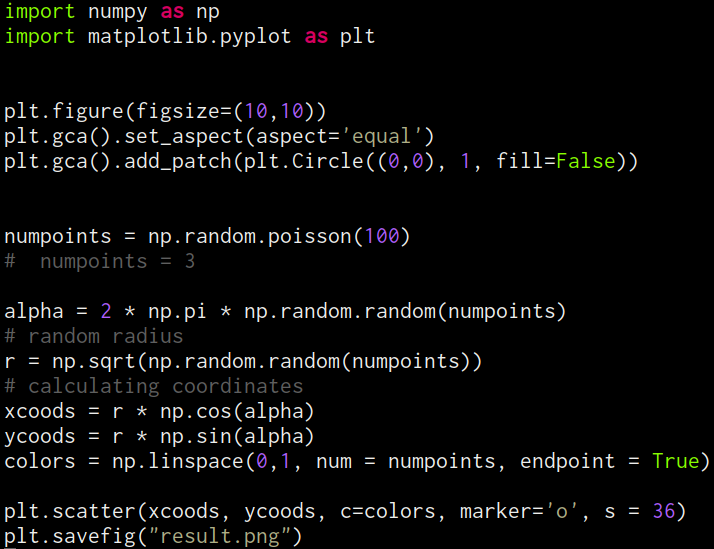
\includegraphics[width=0.5\linewidth]{image/code.png}
\end{figure}
    \item Explanation
        \begin{itemize}
            \item We first simulate $n$ points from a Poisson process with $\lambda = 100$
            \item We then unifomly sample $n$ points uniformly in the 3D space
        \end{itemize}
    \item Result:
\begin{figure} [H]
    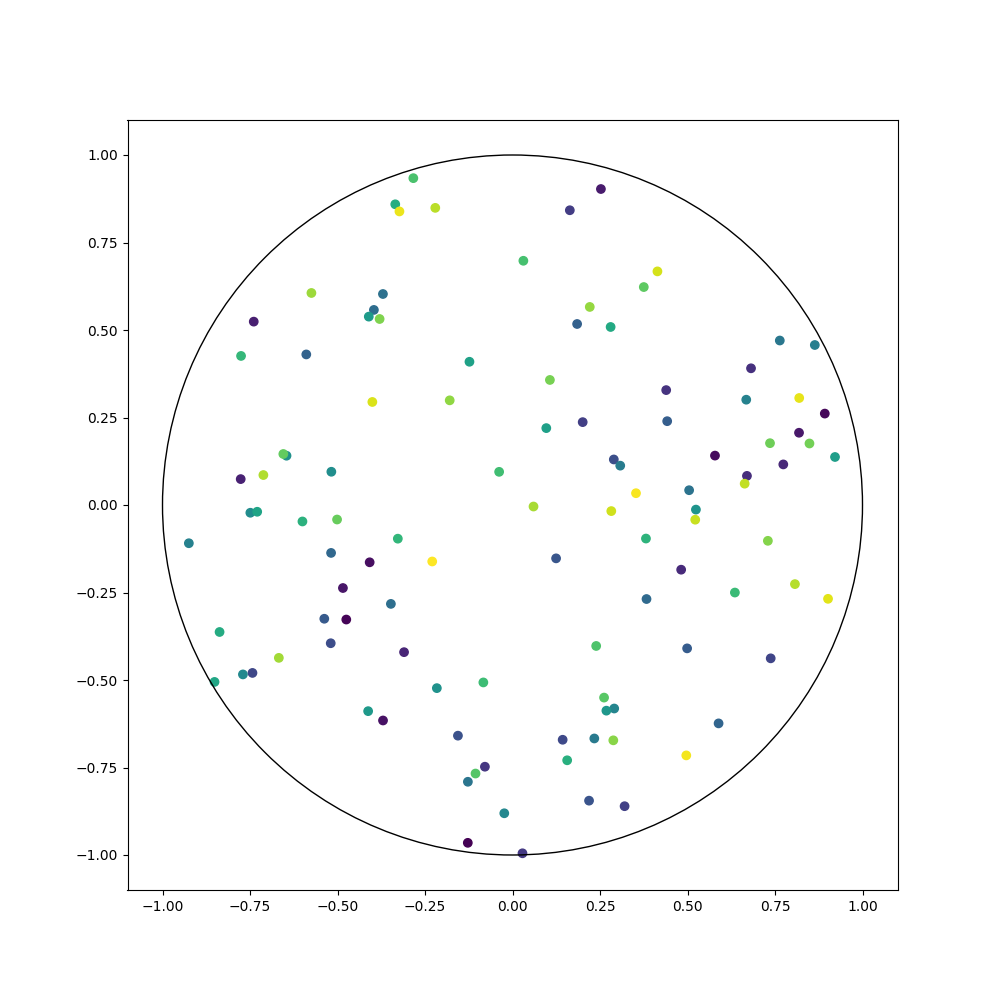
\includegraphics[width=0.5\linewidth]{src/result.png}
\end{figure}
\end{itemize}

\end{document}
